\topicFramePrimary{Real time 3D-PTV technical challenges}

\begin{frame}[label=real-1]{It was pretty heavy laboratory system - ETH Zurich, 1989}
    \centering\cardImg{eth_zurich_3d_ptv_1989}{\textwidth}
\end{frame}

    
\begin{frame}[label=real-2]{With advance of cameras and electronics it only grew in size}
    \centering\cardImg{lab.jpg}{.85\textwidth}
\end{frame}

\begin{frame}[label=real-3]{The high-speed imaging and recording requires literally ``heavy lift''}
\begin{multicols}{2}
    \cardImg{ptv_drives1}{.45\textwidth}
    \cardImg{ptv_drives2}{.45\textwidth}
\end{multicols}
\begin{cardTiny}
    Data transfer rate requires 72 fiber-connected hard drives
\end{cardTiny}
\end{frame}


% \begin{frame}[label=real-5]{We had a dream: 3D-PTV for large scale systems}
% \centering\cardImg{car_ptv.png}{.8\textwidth}
% \end{frame}

% \subsubsection*{Real time image acquisition and processing}
%\begin{frame}{The solution}
%\begin{card}
%\end{card}
%\end{frame}


\begin{frame}[label=real-4]{For instance for 1 min run at 1 kHz we need:}
    \begin{card}[Data transfer rate and size]
    \begin{itemize}
    \item 1.3 Mb/frame $\times$ 1000 frames/sec = 1300 Mb/sec
    \item 1300 Mb/s $\times$ 4 cameras = 5.2 Gb/sec
    \item SSD disk continuous writing speed is about 3.5 Gb/sec
    \item Total data size: 5.2 Gb/sec $\times$ 60 $\approx$ 300 Gb
    \end{itemize}

    \end{card}
\end{frame}

\begin{frame}[label=real-5a]{First attempts tried image compression, similar to G. Voth}
    %\begin{multicols*}{2}
    % \cardImg{realtime1}{.49\textwidth}
    \centering\cardImg{voth}{.8\textwidth}
    % \cardImg{mikrotron_sobel}{.49\textwidth}
    % \cardImg{mikrotron_inside}{.49\textwidth}
    %\end{multicols*}
\end{frame}


\begin{frame}[label=real-5b]{We could utilize the special hardware from Mikrotron }
    \begin{multicols*}{2}
    \cardImg{mikrotron_sobel}{.45\textwidth}
    \cardImg{mikrotron_inside}{.45\textwidth}
    \end{multicols*}
    \centering \cardImg{realtime1}{.8\textwidth}
\end{frame}


\begin{frame}[label=real-6]{It was a significant step forward: real time detection, $x^{(i)},y^{(i)}$ only}
    \centering\cardImg{sobel_1}{.8\textwidth}
\end{frame}


\begin{frame}[label=real-7]{Worked very well for well-controlled laboratory experiments only}
    \begin{card}
    \centering
    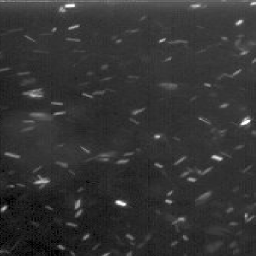
\includegraphics[width=.32\textwidth]{1_in}
    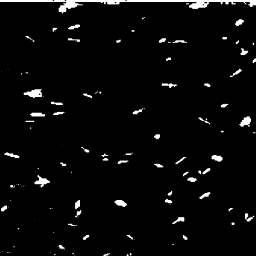
\includegraphics[width=.32\textwidth]{1_binarized}
    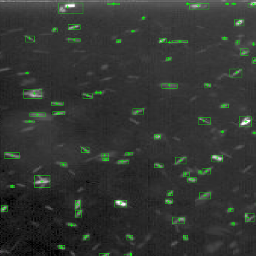
\includegraphics[width=.32\textwidth]{1_out}
    \end{card}
    \vspace{-.5cm}
    \begin{cardTiny}
    Raw image - binary image - blobs marked on the original image.  
    \end{cardTiny}
\end{frame}


\begin{frame}[label=real-7c]{Standard FPGA cameras from Zhao et al. at UIUC}
    \begin{card}[With simple background and large particles it is even simpler]
    \centering
    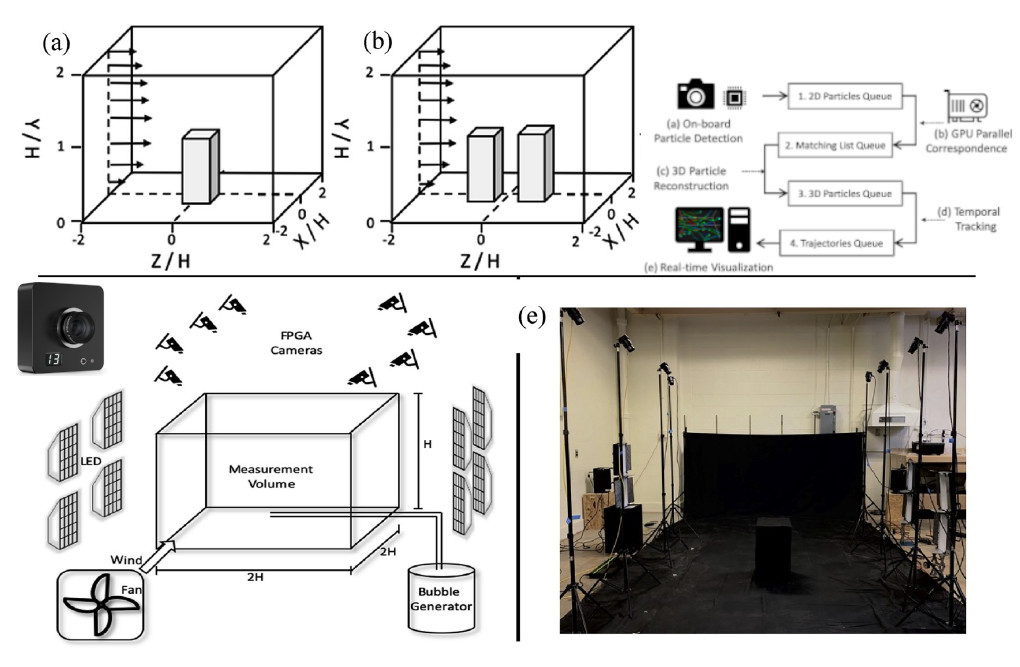
\includegraphics[height=.8\textheight, width=\textwidth, keepaspectratio]{3d_vptv_experiment}
    \end{card}
\end{frame}


\begin{frame}[label=real-8]{Real experiments are more complicated than just a bright dots on a black uniform gradient}
    \begin{multicols}{2}
    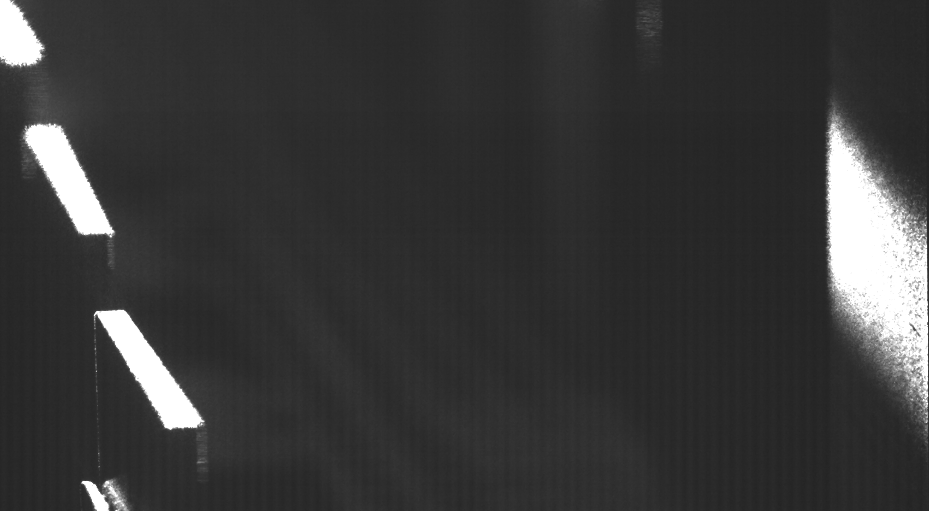
\includegraphics[width=.49\textwidth]{background.png}
    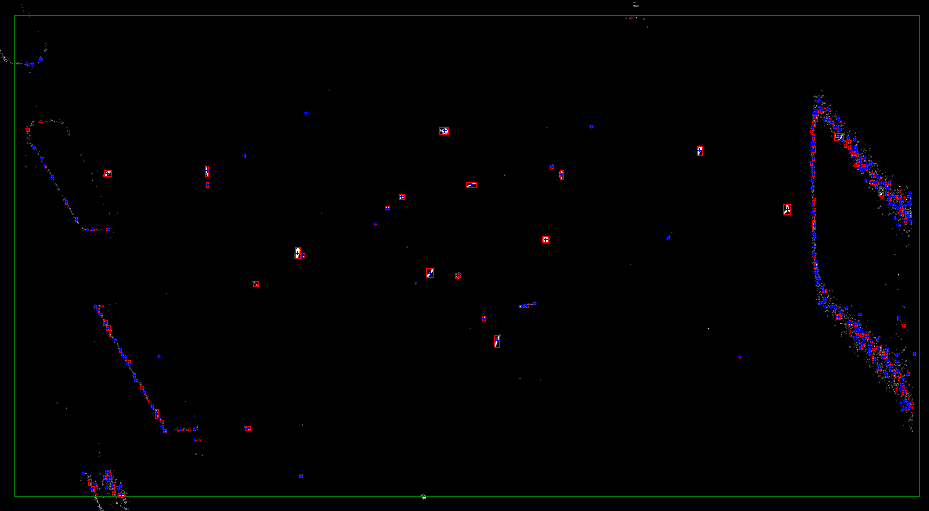
\includegraphics[width=.49\textwidth]{detection.png}
    \end{multicols}
    \begin{cardTiny}
    Raw 3D-PTV image of the wind tunnel experiments: Background ->  binary image after background subtraction, and detection using a locally adaptive filter
    \end{cardTiny}
\end{frame}


\begin{frame}[label=real-10]{Developed a custom image processing (!) algorithm on FPGA}
    \centering\cardImg{fig8}{1\textwidth}
    % \begin{cardTiny} Diagram of the blob analysis algorithm. \end{cardTiny}
    \end{frame}

    \begin{frame}[label=real-11]{1Vision implementated it on SiliconSoftware FPGA framegrabbers}
    \cardImg{1vision_blob_recorder_2}{1\textwidth}
    % \cardImg{backside}{.25\textwidth}
\end{frame}

\begin{frame}[label=real-12]{The main concept}
    \centering\cardImg[height]{fig1.png}{.7\textwidth}
\end{frame}


\begin{frame}[label=real-9]{Together with 1Vision LTD we developed a breakthrough solution on FPGA framegrabbers from Silicon Software GmbH}
    \centering\cardImg{1vision}{1\textwidth}
\end{frame}


% \begin{frame}[label=real-7d]{Future FPGA could include a neural network, Gim et al. at SKKU/KAIST}
%     %\begin{card}{Convolutional neural network}
%     \centering \cardImg[height=.8\textheight]{3d_detection_cnn}{\textwidth}
% \end{frame}



%\end{document}